\chapter{Теоритическая часть}\label{ch:-}


\section{Системы автоматической сборки}

В свете быстрого развития современных информационных технологий и повышенных требований к
эффективности программных систем, внедрение интегрированных средств автоматизации сборки является
неотъемлемым этапом в процессе разработки программного обеспечения.
В данной главе рассматривается
важная составляющая инфраструктуры разработки - интеграция системы автоматической сборки в
контексте платформы аналитики исторических данных с использованием микросервисной архитектуры.

Gradle представляет собой мощный инструмент для автоматизации процессов сборки и управления
зависимостями в проектах различной сложности.
Его гибкость и расширяемость позволяют эффективно
управлять процессом сборки как небольших приложений, так и крупных программных комплексов.
В
контексте платформы аналитики исторических данных, где требуется обеспечить высокую
производительность и надежность при обработке больших объемов информации, внедрение Gradle
представляется важным шагом для оптимизации процесса разработки и поддержки программного
обеспечения.

Данная глава направлена на анализ методов интеграции системы автоматической сборки Gradle
в существующую инфраструктуру обслуживания микросервисов платформы аналитики исторических данных.
В
частности, рассматриваются вопросы настройки Gradle для удовлетворения требований по сборке,
тестированию и развертыванию микросервисов, а также оптимизации процесса разработки и управления
зависимостями.
Предполагается, что результаты данного исследования смогут служить основой для
разработки эффективной и масштабируемой инфраструктуры сборки в рамках платформы аналитики
исторических данных, способствуя повышению производительности и надежности разрабатываемых
приложений.

\subsection{Обоснование выбора Gradle}

В данном разделе обосновывается выбор системы автоматической сборки Gradle в качестве основного инструмента для интеграции в инфраструктуру разработки на платформе аналитики исторических данных.
Рассматриваются основные преимущества и функциональные возможности Gradle, а также адаптация данной системы к требованиям и особенностям разрабатываемого программного комплекса.
Рассматриваются факторы, влияющие на принятие данного решения.

\subsubsection{Системы автоматизированных сборок}

Gradle — это система автоматизации сборки с открытым исходным кодом, в которой используются те же идеи, что и в Apache Maven и Apache Ant.
Он использует предметно-ориентированный язык, основанный на компьютерном языке Groovy или Kotlin, в отличие от Apache Maven, настройка проекта которого использует XML~\cite{gradle_vs_maven}.

\subsubsection{Основные различия}

Существуют существенные различия в подходах к построению двух систем.
Gradle основан на модели сети зависимостей задач, где каждая задача представляет собой исполняемый объект, выполняющий определенные действия.
В отличие от этого, в Maven стадии проекта связаны с целями, которые функционируют аналогично задачам в Gradle как объекты, осуществляющие выполнение работы.

\subsubsection{Производительность}

Оба фреймворка обеспечивают возможность одновременного выполнения множества сборок модулей с учетом аспектов производительности.
Gradle, в частности, обладает возможностью проведения инкрементных сборок, так как он способен определить, какие задачи были изменены.
Кроме того, Gradle обладает рядом выдающихся характеристик производительности, среди которых следует выделить:

\begin{enumerate}
    \item Инкрементальная компиляция классов Java, что позволяет значительно сократить время сборки за счет перекомпиляции только тех классов, которые были изменены.
    \item Компиляция предотвращения для Java, предоставляющая возможность быстрого обнаружения ошибок в коде на этапе компиляции.
    \item API для дополнительных подзадач, что обеспечивает гибкость в настройке и расширении процесса сборки.
    \item Демон компилятора, который значительно ускоряет процесс компиляции за счет сохранения в памяти некоторых результатов предыдущих компиляций.
\end{enumerate}

На рисунке~\ref{fig:performance_comparison}представлен сравнительный тест производительности автоматизированной сборки одинаковых проектов и прохождение тестов~\cite{detailed_comprasion}.

\begin{figure}[htbp]
    \centering
    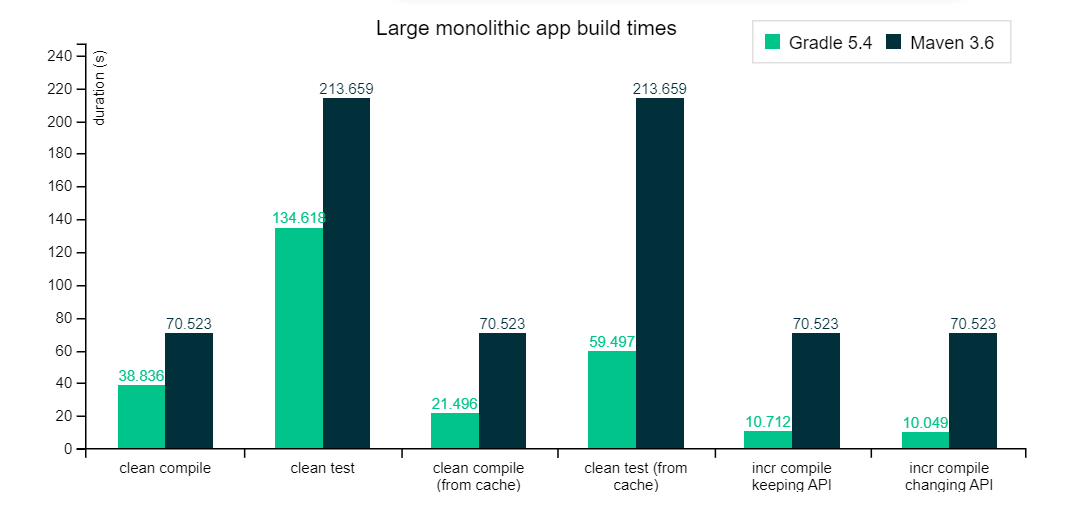
\includegraphics[width=0.8\textwidth]{gradle_perfomance}
    \caption{Сравнительный тест производительности}
    \label{fig:performance_comparison}
\end{figure}


\section{API Gateway. Маршрутизация и фильтрация}

В нынешних стандартах информационных технологий существует понятие цифровой экосистемы, требующей
эффективной обработки и управления потоком данных.
В контексте цифровой экосистемы появляется
надобность в инструментарии, способном на рационализацию и организацию потока данных между
клиентами и целевыми микросервисами.
API Gateway становится одним из важных решений в данном
контексте.

API Gateway -- инструмент, предоставляющий функциональность машрутизации, фильтрации и авторизации
трафика.
Он является одним из важных компонентов в рамках микросервисной архитектуры,
способствующий организации внутренних и внешних взаимодействий между компонентами системы.

\subsection{Прямое взаимодействие клиента и сервиса}

В контексте современных подходов к разработке миркосервисных платформ в некоторых случаях
рассматривается возможность прямого взаимодействия клиента с микросервисом.
Этот подход
предполагает, что клиентское приложение
способно напрямую отправлять запросы к отдельным микросервисам без посредника между ними.
В данном
сценарии, каждый микросервис предоставляет общедоступный эндпоинт, часто с индивидуальным
TCP-портом, что обеспечивает прямой доступ к конкретному сервису~\cite{trebichavsky2021api}.

При таком подходе первостепенно возникает необходимость в прозрачном механизме для управления
трафиком и обеспечения безопасности
взаимодействия между клиентом и микросервисами.
В данном контексте, могут быть задействованы
дополнительные
инструменты, например балансировщики нагрузки или ADC, которые помогают
обеспечить не только равномерное распределение запросов между микросервисами, но и обеспечивают
уровень базовый уровень защиты, к примеру использование при запросах
протокола SSL для шифрования соединения.

Однако, при создании масштабных приложений на основе микросервисов, особенно при взаимодействии с
удаленными мобильными приложениями или веб-приложениями SPA, сталкиваются с
рядом множественных вызовов.
При увеличении системы
вызовы требуют минимизации обращений к серверной части для сокращений задержки обращения и расходов
на эксплотацию,
управление сквозными задачами, такими как авторизация и безопасность, а также создание
специализированных дополнительных фасадов для оптимизации работы и разделение бизнес-логики для
различных типов клиентских приложений~\cite{ApiGatewayDirect}.

Следовательно, в контексте архитектуры прямого взаимодействия клиент-микросервис, важно учитывать не
только технологические аспекты, но и сложившиеся практики и вызовы, с которыми сталкиваются
разработчики при проектировании и развертывании современных цифровых приложений.

Пример прямой связи клиента и сервиса представлен на рисунке~\ref{fig:direct_link}

\begin{figure}[htbp]
    \centering
    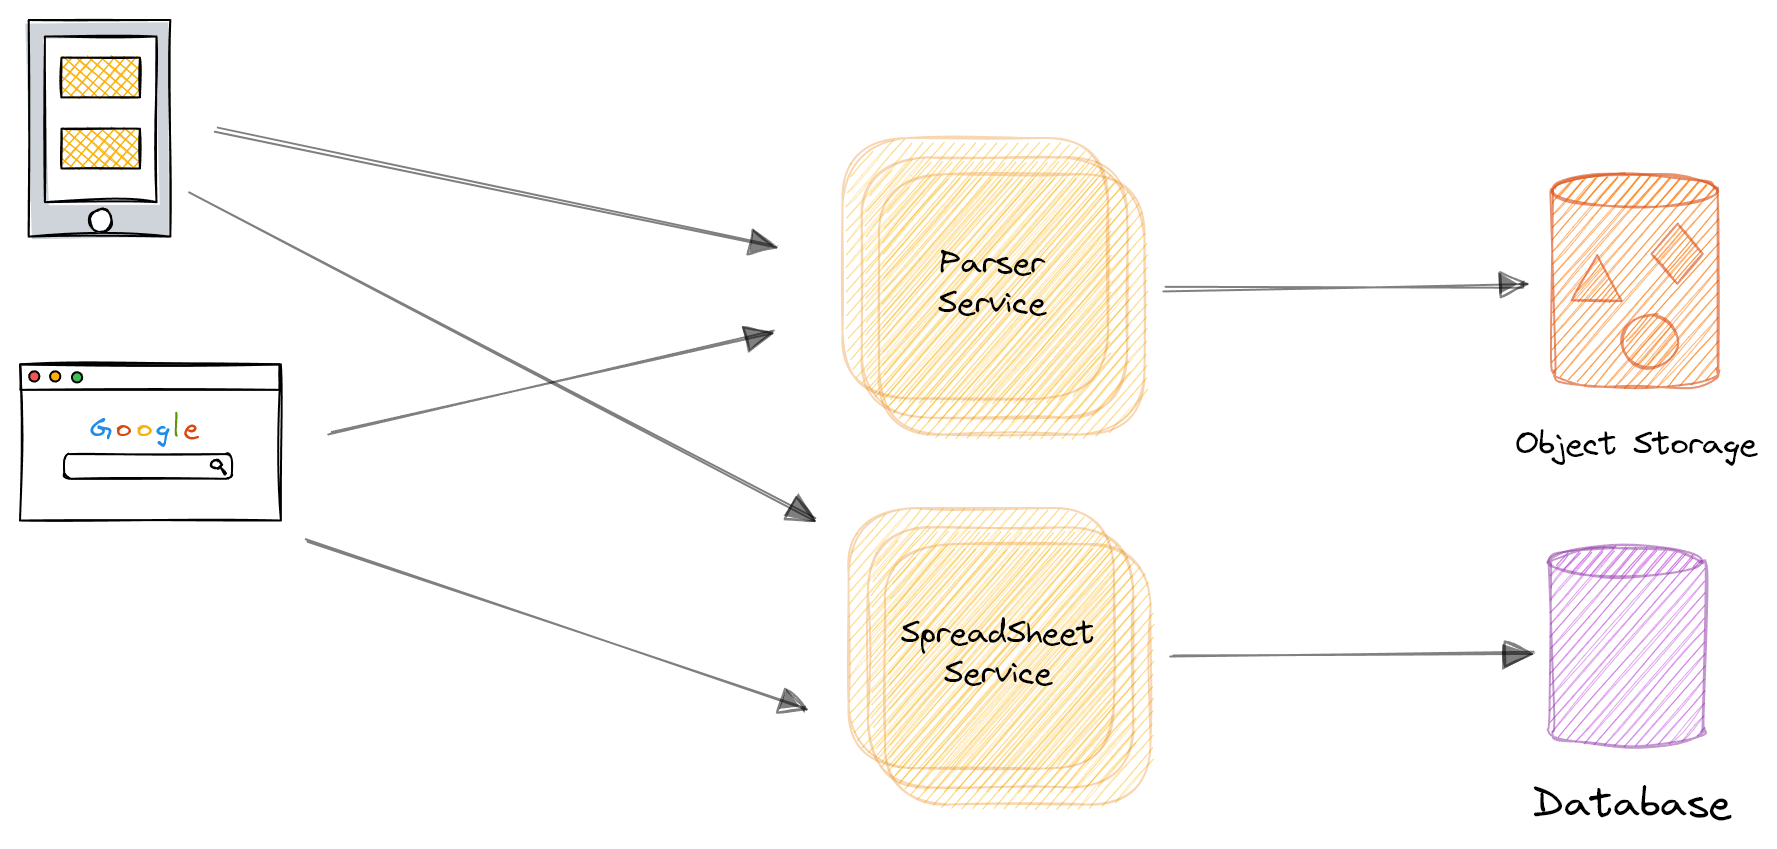
\includegraphics[width=0.8\textwidth]{direct_link}
    \caption{Прямая связь клиента и сервиса}
    \label{fig:direct_link}
\end{figure}

\subsubsection{Проблемы подхода}

Следует учитывать, что при прямом соединении клиента и отдельных сервисов нелинейно увеличивается
сложность взаимодействия и управления.
Связанно это с необходимостью поддержания соединения с
клиентом на протяжении всего запроса, что потенциально увеличивает нагрузку на ресурсы сети.

Ко всему такой подход несет серьезные проблемы с безопасностью, так как отсутствует
централизированный
механизм контроля аунтефикации.
Эта проблема несет за собой, в том числе и проблемы поддержания
единого соглашения политики безопасности сервиса из-за необходимости каждого отдельного сервиса
обеспечивать собственную безопасность.

Наконец, прямое взаимодействие усложняет обновление и масштабирование системы.
При внесении
изменений в микросервисы или добавлении новых компонентов необходимо обновлять каждое клиентское
приложение, что может быть трудоемким и время затратным процессом.

\subsection{Api Gateway}

Шаблон API Gateway представляет собой концепцию, используемую при разработке и архитектуре
масштабных или комплексных приложений, основанных на архитектуре микросервисов и включающих
несколько клиентских приложений.
В контексте данной практики API Gateway представляет собой сервис,
который функционирует как централизованная точка входа для определенных кластеров микросервисов.
Этот шаблон, аналогичный концепции фасада в объектно-ориентированном проектировании, является
составной частью децентрализованных систем~\cite{zhao2018management}.

Следовательно, API Gateway размещается между клиентскими приложениями и микросервисами, действуя в
качестве обратного прокси-сервера, который маршрутизирует запросы от клиентов к соответствующим
сервисам.
Тем не менее API Gateway обеспечивает дополнительную функциональность, такую как
аутентификация, SSL и кэширование.

На рисунке~\ref{fig:link_with_gate} представлена диаграмма, иллюстрирующая интеграцию
пользовательского
API Gateway в упрощенную схему архитектуры микросервисов.

\begin{figure}[htbp]
    \centering
    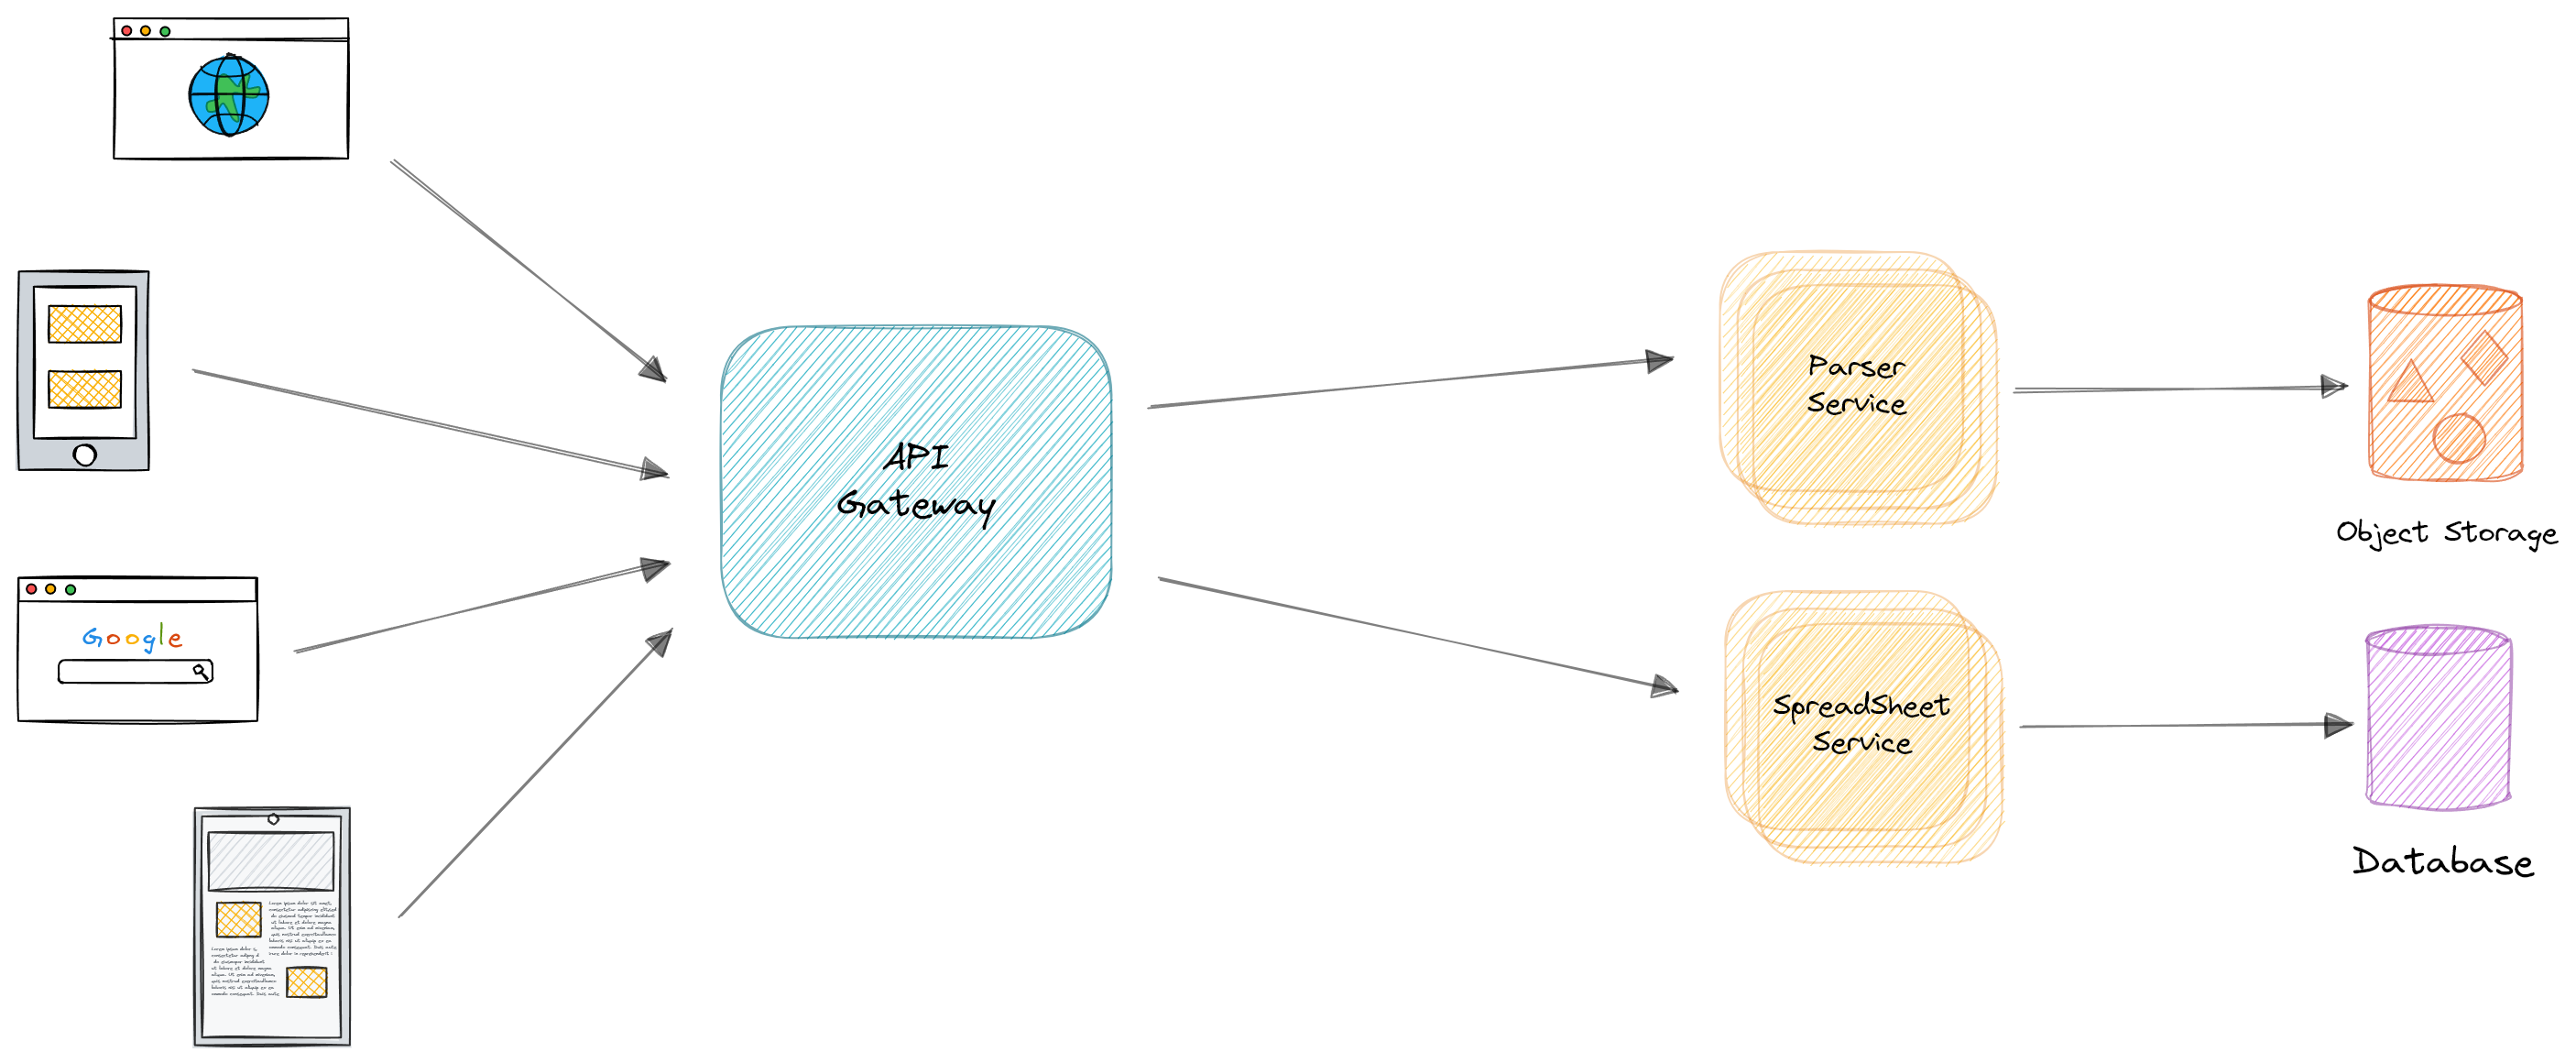
\includegraphics[width=0.8\textwidth]{link_with_gateway}
    \caption{Связь через API Gateway}
    \label{fig:link_with_gate}
\end{figure}

Важно подчеркнуть, что в представленной схеме используется единый пользовательский сервис API
Gateway, обслуживающий несколько различных клиентских приложений.
Это может представлять риск в
плане масштабирования и поддержки, так как сервис API Gateway становится весьма сложным из-за
разнообразных требований клиентских приложений.
Это может привести к его увеличению и, в конечном
итоге, превращению в монолитное приложение или сервис.
Следовательно, рекомендуется разделение API
Gateway на несколько служб или отдельных API Gateways в соответствии с бизнес-границами и
потребностями клиентских приложений.

Разработка и реализация API Gateway требует осторожного подхода.
Объединение всех внутренних
микросервисов приложения в единый API Gateway может привести к нарушению автономии микросервисов и
созданию архитектурного оркестратора, что не рекомендуется.

\subsubsection{BFF}

При разделении уровня API Gateway на несколько компонентов, например, при наличии нескольких
клиентских приложений, основным руководством является создание различных эндпоинтов API Gateways в
соответствии
с типами клиентов.
Это может быть реализовано через применение шаблона <<Серверная часть для
интерфейса>> (BFF), где API Gateway предоставляет специализированный API для конкретного типа
клиентского приложения~\ref{fig:bff_gate}.

\begin{figure}[htbp]
    \centering
    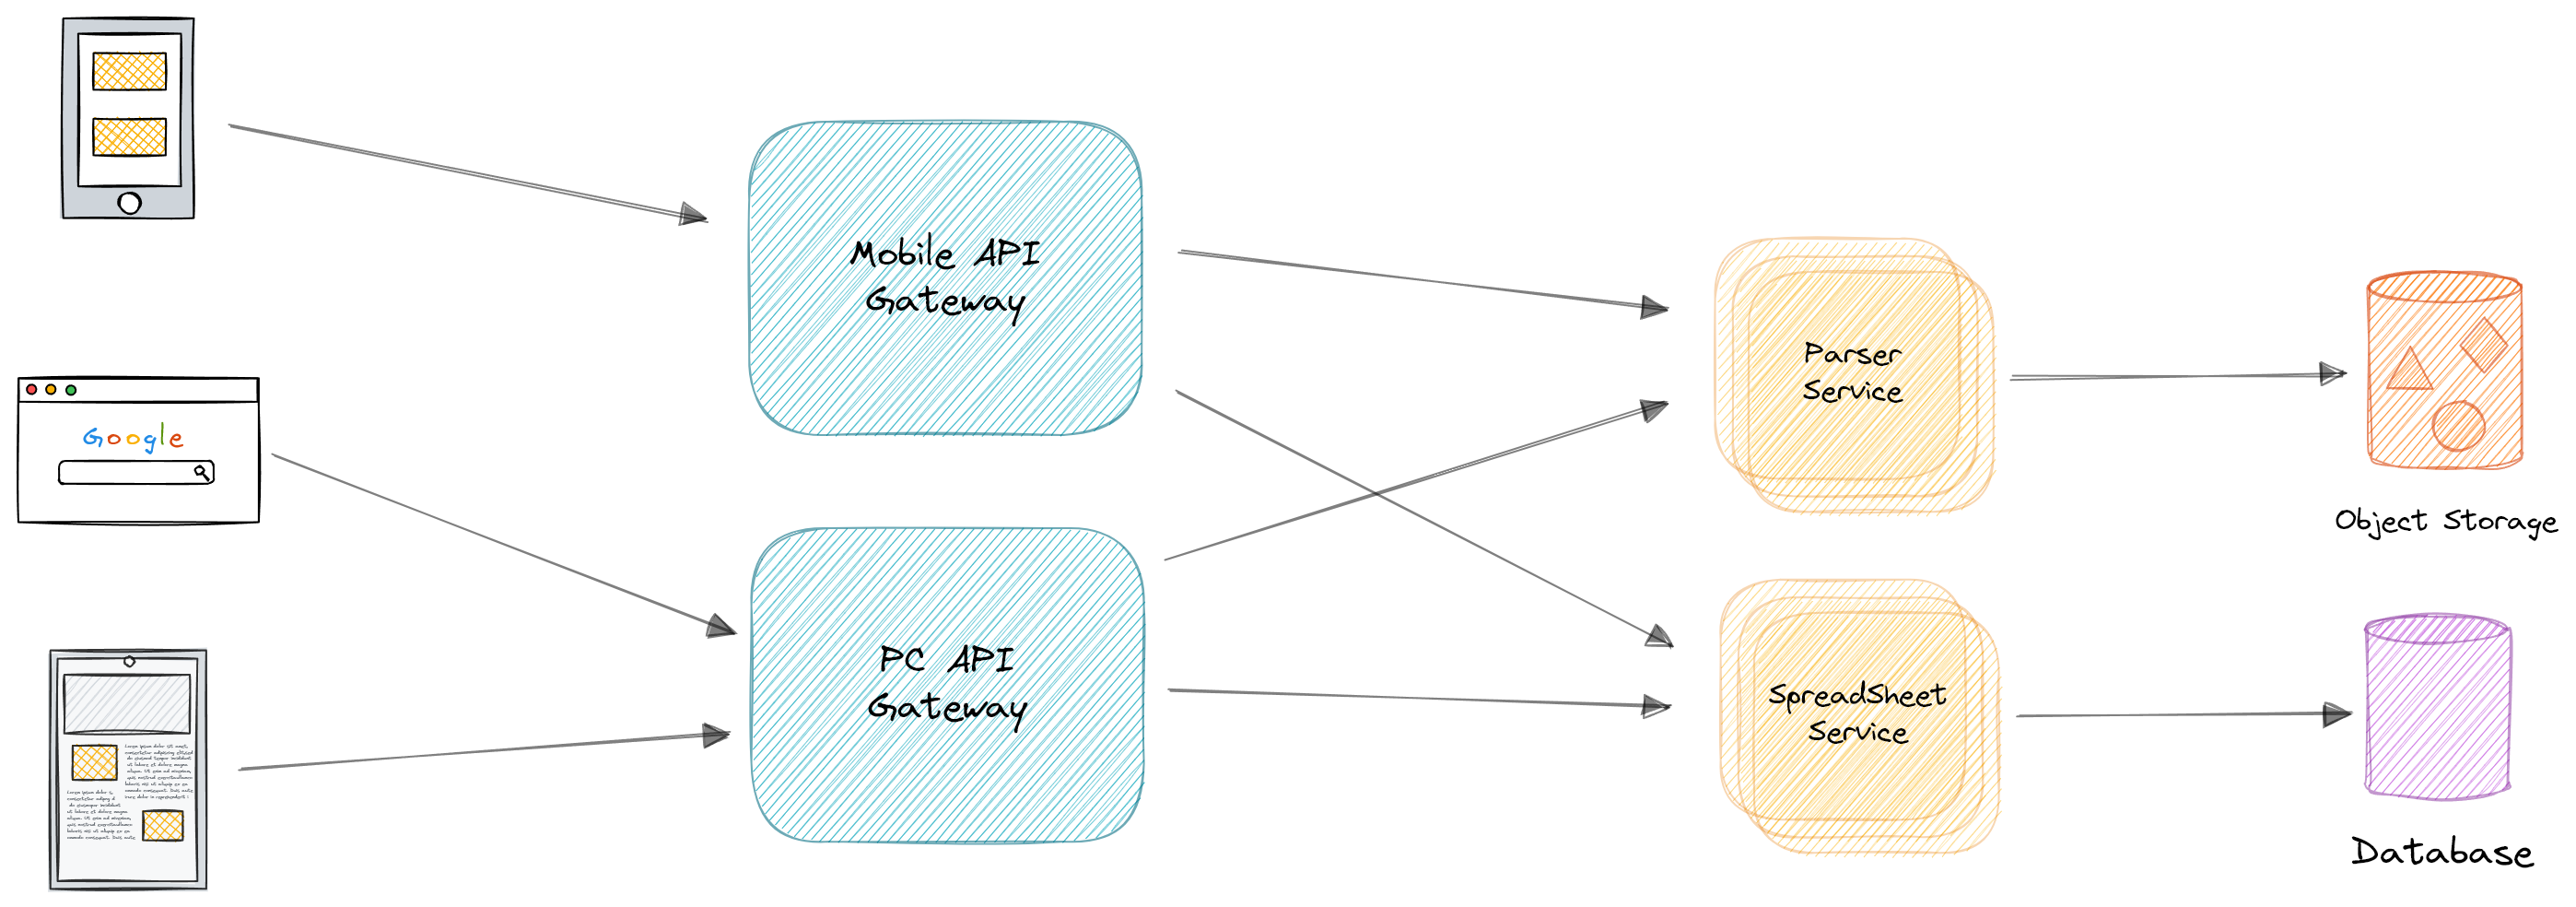
\includegraphics[width=0.8\textwidth]{BFF_gateway}
    \caption{BFF}
    \label{fig:bff_gate}
\end{figure}

Для платформ, использующих множество сервисов, важность применения агрегации возрастает, так как
требуется объединение нескольких низкоуровневых вызовов для обеспечения пользовательских функций~\cite{alkhodary2023evaluation}.
В
таких сценариях один вызов к шлюзу для фронтендов (BFF) обычно порождает ряд низкоуровневых вызовов
к разным микросервисам.
Примером может послужить приложение для аналитики исторических данных, в
котором
пользователь требует получения списка координат церквей из определенного уезда для визуализации
движения рукописи
за определенный период времени.

С точки зрения оптимизации ресурсов было бы целесообразно осуществлять как можно больше вызовов
параллельно.
После завершения начального вызова к сервису <<Поиска координат>> оптимально выполнять
вызовы других сервисов параллельно, с целью сократить общее время обработки~\cite{BFF}.
\ref{fig:parrallel_query}
\begin{figure}[htbp]
    \centering
    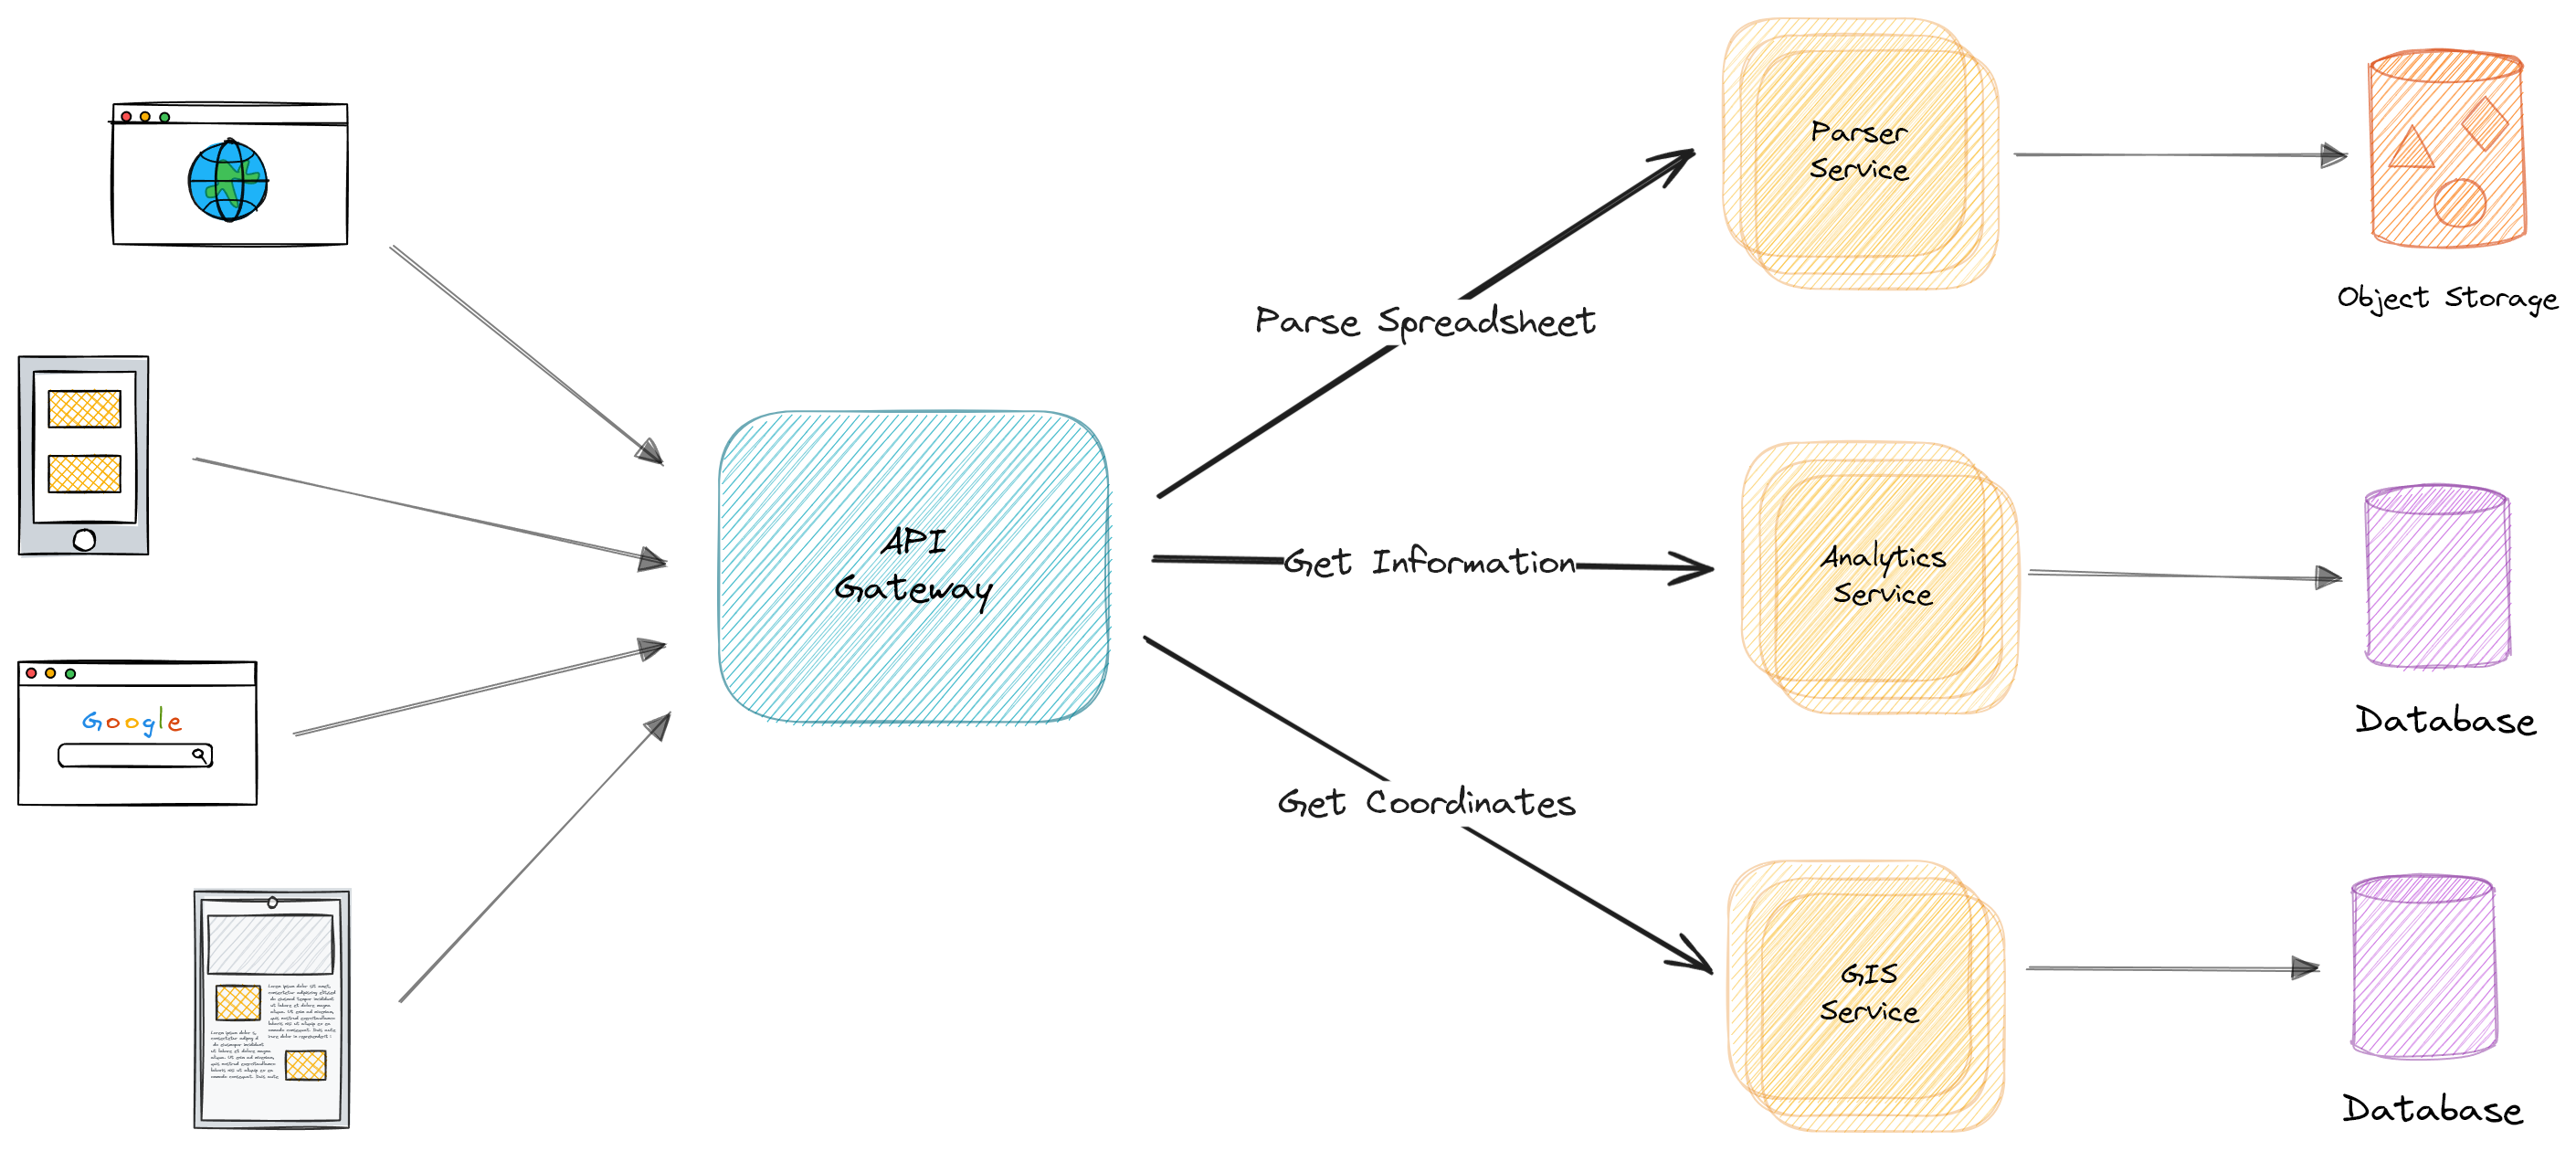
\includegraphics[width=0.8\textwidth]{parallel_query}
    \caption{BFF}
    \label{fig:parrallel_query}
\end{figure}

\subsection{Сравнение популярных решений}

Для сравнения API Gateway необходимо определить критерии, по которым будут оцениваться различные решения.
Основные
критерии включают производительность, масштабируемость, безопасность, интеграцию с другими сервисами, удобство настройки
и использования, а также сообщество и поддержку.

Сравниваемые решения включают:
\begin{itemize}
    \item Spring Cloud Gateway
    \item Kong
    \item Amazon API Gateway
    \item Apigee
    \item NGINX

\end{itemize}

\subsubsection{Производительность}

Spring Cloud Gateway демонстрирует высокую производительность благодаря реактивной архитектуре на основе проекта Spring
WebFlux.
Это обеспечивает асинхронную обработку запросов и высокую пропускную способность.

Kong также имеет высокую производительность благодаря использованию NGINX и LuaJIT, что позволяет обрабатывать тысячи
запросов в секунду с низкой задержкой.

Amazon API Gateway интегрирован с AWS инфраструктурой, обеспечивая надежную и масштабируемую производительность.
Однако,
для достижения высокой производительности могут потребоваться дополнительные настройки и использование AWS Lambda.

Apigee обладает хорошей производительностью, однако может уступать в сценариях с высокими нагрузками по сравнению с
решениями на основе NGINX\@.

NGINX известен своей высокой производительностью и низкой задержкой, что делает его популярным выбором для API Gateway.

\subsubsection{Масштабируемость}

Spring Cloud Gateway легко масштабируется в рамках экосистемы Spring Cloud, поддерживая кластеризацию и интеграцию с
различными системами оркестрации, такими как Kubernetes~\cite{carnell2021spring}.

Kong поддерживает горизонтальное масштабирование и интеграцию с различными оркестраторами контейнеров, что делает его
подходящим для крупных распределённых систем.

Amazon API Gateway предлагает автоматическое масштабирование в рамках AWS, что позволяет обрабатывать любые объемы
трафика без необходимости управления инфраструктурой.

Apigee предоставляет масштабируемость на уровне предприятия, поддерживая гибкость и высокую доступность.

NGINX, как и Kong, легко масштабируется горизонтально, что позволяет его использовать в крупных распределённых системах.

\subsubsection{Безопасность}

Spring Cloud Gateway поддерживает интеграцию с различными решениями для аутентификации и авторизации, такими как OAuth2
и JWT, а также предоставляет возможности для настройки правил безопасности.

Kong обладает мощными функциями безопасности, включая аутентификацию, авторизацию, SSL/TLS шифрование и контроль доступа
на уровне API\@.

Amazon API Gateway интегрируется с AWS IAM для управления доступом, а также поддерживает API ключи, OAuth и
пользовательские авторизационные механизмы.

Apigee предлагает широкий набор функций безопасности, включая шифрование, управление доступом и интеграцию с системами
аутентификации.

NGINX обеспечивает базовые функции безопасности и поддерживает расширенные настройки через модули и интеграции с другими
решениями безопасности.

\subsubsection{Интеграция с другими сервисами}

Spring Cloud Gateway тесно интегрирован с экосистемой Spring, что обеспечивает простую интеграцию с микросервисами и
другими компонентами на базе Spring.

Kong поддерживает интеграцию с различными базами данных, системами мониторинга и логирования, а также предоставляет
множество плагинов для расширения функциональности.

Amazon API Gateway интегрируется с различными сервисами AWS, такими как Lambda, DynamoDB, S3 и другие, что делает его
мощным инструментом для построения серверлесс-приложений.

Apigee предлагает интеграцию с различными облачными платформами и сервисами, а также поддерживает гибкие возможности
расширения через API и SDK\@.

NGINX может интегрироваться с различными сервисами через модули и конфигурации, обеспечивая гибкость в построении
сложных инфраструктур.

\subsubsection{Удобство настройки и использования}

Spring Cloud Gateway предоставляет декларативный способ настройки через YAML или Java-код, что делает его удобным для
разработчиков, знакомых с экосистемой Spring.

Kong предлагает интуитивно понятный интерфейс и мощный API для управления конфигурациями, что упрощает его настройку и
использование.

Amazon API Gateway предоставляет удобный веб-интерфейс и API для управления, но может потребовать времени на освоение
всех возможностей и особенностей настройки в контексте AWS\@.

Apigee предлагает мощный интерфейс для управления API и инструментами аналитики, что облегчает процесс настройки и
мониторинга.

NGINX требует глубокой настройки через конфигурационные файлы, что может потребовать значительных усилий для оптимальной
настройки и управления.

\subsubsection{Сообщество и поддержка}

Spring Cloud Gateway пользуется поддержкой большого сообщества разработчиков Spring, что обеспечивает доступ к обширной
документации, форумам и ресурсам.

Kong имеет активное сообщество и предоставляет коммерческую поддержку через Kong Enterprise.

Amazon API Gateway получает поддержку от AWS, включая обширную документацию, обучающие материалы и техподдержку.

Apigee обладает сильной поддержкой от Google, включая документацию, обучающие материалы и коммерческую поддержку.

NGINX имеет большое сообщество пользователей и разработчиков, а также коммерческую поддержку через NGINX Plus.

\subsubsection{Вывод}

Spring Cloud Gateway, благодаря своей высокой производительности, простоте интеграции с экосистемой Spring, мощным
возможностям настройки и широкому сообществу, является предпочтительным выбором для проектов, использующих стек
технологий Spring.
Он обеспечивает гибкость, масштабируемость и безопасность, необходимые для современных микросервисных
архитектур, и, таким образом, заслуженно выходит победителем в этом сравнении.

\subsection{Spring Cloud Gateway}

Для проекта платформы аналитики исторических данных перед API Gateway выдвигаются определенные
требования:
\begin{enumerate}
    \item  Должен маршрутизировать запросы в различные модификации сервисов в зависимости от клиента.
    \item Поддержка Oauth 2.0 для передачи информации о пользователи в API сервисы
    \item Метрики для оценки загрузки сервиса и задержки ответов.
    \item Логирование запросов и ответов.
\end{enumerate}



Spring Cloud Gateway успешно справляется со всеми выдвигаемыми требованиями.
Тем не менее его важное преймущество -- работа в режиме non-blocking.

\subsubsection{Non-blocking Spring Cloud Gateway}

Неблокирующая схема, реализованная вне контекста сервлетов и функционирующая на основе Netty,
основанного на проекте Reactor, представляет собой асинхронный фреймворк, ориентированный на event
loop'ы, а не на статически определенное количество потоков.
В данной схеме может
присутствовать только один поток.
Каждый процессорный поток управляет одной петлей, в которой
сосредоточены каналы, принимающие входящие TCP-соединения, декодирующие HTTP-запросы (это происходит
быстро) и передающие их дальше.

Запрос поступает через HTTP в канал, затем через петлю событий и далее в приложение WebFlux (реактивный подход к написанию приложений Spring, основанный на Project Reactor) в виде объекта
ServerHttpRequest - нового объекта, заменяющего HttpServletRequest.
Это происходит неблокирующим
образом: петля событий получает событие из канала, обрабатывает его, создает флаг ожидания
ответа, отправляет его дальше по цепочке и готова снова принимать запросы.
WebFlux оборачивает его в
ServerWebExchange, который содержит в себе и запрос, и ответ, и передает их дальше по цепочке до
WebClient - того же HttpClient, но способного работать асинхронно.

Таким образом, получается аналог контекста сервлетов, но уже работающий в неблокирующем режиме, с
использованием реактивных операторов.
Ко всему же, все происходит асинхронно, так что даже при
наличии только одного процессорного потока все будет
функционировать~\cite{spirng_gateway}.

\subsubsection{Circuit breaker pattern}

В процессе обработки запросов микросервсисы часто взаимодействуют друг с другом.
Когда один сервсис
синхронно вызывает другой, существует вероятность того, что второй сервис будет недоступна или его
задержка будет настолько велика, что пользование им станет практически невозможным.
Это может
привести к неэффективному использованию ресурсов, например, потоков, которые могут быть
заблокированы вызывающей стороной в ожидании ответа от другой службы.
Такие ситуации могут привести
к истощению ресурсов и, в конечном итоге, вызвать неспособность обработки других запросов вызывающей
службой.
Кроме того, сбой одной службы может потенциально повлиять на работу других служб в рамках
всего приложения~\cite{circuit_breaker}.

Встает вопрос о необходимости предотвращения распространения сбоев одних сервисов на другие.

Для обеспечения взаимодействия клиента службы с удаленной службой необходимо использовать
прокси-сервер, функционирующий по аналогии с электрическим выключателем.
При достижении
определенного порогового значения последовательных сбоев происходит автоматическое срабатывание
выключателя.
В течение установленного периода ожидания все попытки обращения к удаленной службе
завершаются неудачей.
По истечении данного времени автоматический выключатель пропускает
ограниченное количество тестовых запросов.
В случае успешного завершения данных запросов выключатель
восстанавливает нормальный режим работы.
Однако, если тестовые запросы завершаются неудачно,
происходит повторный запуск периода ожидания, и цикл
возобновляется~\cite{microservice_pattern}.

Такой подход имеет и минусы из-за неправильного подбора значения тайм-аута из-за чего в следствии
создаются ложные срабатывания и дополнительные задержки.


\section{Сервер конфигураций}

Внедрение сервера конфигурации в инфраструктуру микросервисов обладает значительной важностью, что обусловлено рядом
факторов, влияющих на стабильность, управляемость и масштабируемость систем~\cite{carnell2021spring}.

Во-первых, сервер конфигурации позволяет централизованно управлять настройками множества микросервисов.
В условиях,
когда каждый микросервис может иметь свои уникальные параметры, централизованное управление конфигурациями обеспечивает
консистентность и согласованность между различными компонентами системы.
Это особенно критично в распределенных
системах, где конфигурационные изменения должны оперативно и синхронно применяться ко всем компонентам.

Во-вторых, централизованное хранение конфигураций облегчает процесс обновления и развертывания микросервисов.
Внедрение
сервера конфигурации позволяет динамически изменять параметры конфигурации без необходимости перезапуска самих
микросервисов.
Это сокращает время простоя системы и повышает её доступность, что важно для бизнес-критичных приложений.

В-третьих, сервер конфигурации улучшает безопасность системы.
Конфиденциальные данные, такие как ключи API и пароли,
могут храниться в зашифрованном виде и предоставляться только авторизованным микросервисам.
Это снижает риск утечек
данных и упрощает управление доступом к чувствительной информации.

Четвертое значительное преимущество - улучшение масштабируемости.
С ростом количества микросервисов и их экземпляров,
управление конфигурацией становится всё более сложной задачей.
Сервер конфигурации позволяет легко масштабировать
системы, обеспечивая быстрый и гибкий доступ к необходимым параметрам конфигурации независимо от числа микросервисов.

В заключении, внедрение сервера конфигурации способствует лучшей отслеживаемости и управляемости изменений конфигураций.
Введение версионирования конфигурационных файлов позволяет отслеживать историю изменений, что облегчает диагностику и
устранение неполадок.
Это обеспечивает прозрачность и контроль над изменениями в системе, что важно для поддержания её
стабильности и надежности.

Таким образом, сервер конфигурации является одним из ключевых компонентов современной архитектуры микросервисов,
способствующим
повышению эффективности управления, безопасности, масштабируемости и стабильности системы.

\subsection{Выбор сервера конфигурации}

\subsubsection{Критерии выбора сервера конфигурации}

При выборе сервера конфигурации для платформы анализа исторических данных необходимо учитывать ряд ключевых критериев,
которые помогут обеспечить надежную и эффективную работу всей инфраструктуры.

Первым критерием можно выделить необходимость в высокой доступности, то есть сервис должен обладать механизмами
автоматического
восстановления и способностью к горизонтальному масштабированию, чтобы минимизировать время простоя.
Следующим фактором при выборе должна быть способность обеспечения минимальных задержек при доступе к конфиг файлам,
а также возможность поддержки различных форматов файлов, например `json`, `yaml` и другие.

Не стоит забывать и про лицензию для использования.
Необходимо перед использованием ознакомиться с условиями
лицензирования и возможностью использования сервера конфигурации в коммерческих и некоммерческих проектах.

Также должны поддерживаться методы шифрования конфигураций как в состоянии потока, так и при передаче.

Опциональным условием будет наличие активного сообщества разработчиков у проекта, потому наличие такого сообщества,
способно предоставить обновление или улучшение продукта.

\subsubsection{Сравнение популярных решений}

Для сравнения популярных решений для управления конфигурацией и сервисами в распределённых системах рассмотрим три
наиболее часто используемых инструмента: Consul, etcd и Spring Cloud Config.
Каждый из этих инструментов имеет свои
особенности, преимущества и недостатки, которые будут проанализированы в данной теме.

\textbf{Consul}

\textbf{Описание:} Consul — это распределённая система управления конфигурациями, обнаружения сервисов и организации сервисной сети (service mesh), разработанная компанией HashiCorp.
Consul предоставляет функционал для регистрации сервисов, проверки их состояния, распределённого хранения конфигураций и автоматизации сетевого взаимодействия между сервисами.

\textbf{Преимущества:}
\begin{enumerate}[label=\arabic*.]
    \item \textbf{Обнаружение сервисов:} Consul автоматически обнаруживает и регистрирует сервисы, что облегчает управление сложными инфраструктурами.
    \item \textbf{Проверка состояния:} Встроенные механизмы health-check позволяют отслеживать состояние сервисов в реальном времени.
    \item \textbf{Ключ-значение хранилище:} Consul использует KV-хранилище для распределённого хранения конфигураций.
    \item \textbf{Service Mesh:} Consul поддерживает функции сервисной сети, включая управление сетевыми политиками и мидлварное шифрование.
\end{enumerate}

\textbf{Недостатки:}
\begin{enumerate}[label=\arabic*.]
    \item \textbf{Сложность настройки:} Конфигурация и интеграция Consul может быть сложной, особенно в больших кластерах.
    \item \textbf{Ресурсоёмкость:} Требования к ресурсам для поддержания Consul-кластера могут быть высокими, что ограничивает его использование в небольших проектах.
\end{enumerate}


\textbf{etcd}

\textbf{Описание:} etcd — это распределённое хранилище конфигураций, ориентированное на консенсус, разработанное CoreOS. Оно используется в различных системах, таких как Kubernetes, для хранения конфигурационных данных и метаданных.

\textbf{Преимущества:}
\begin{enumerate}[label=\arabic*.]
    \item \textbf{Согласованность данных:} etcd обеспечивает строгое согласование данных благодаря алгоритму Raft.
    \item \textbf{Высокая производительность:} Высокая производительность и низкая задержка доступа к данным.
    \item \textbf{Простота:} Простая и лёгкая в использовании API для операций с данными.
    \item \textbf{Интеграция с Kubernetes:} Является основным хранилищем конфигураций для Kubernetes, что обеспечивает глубокую интеграцию и стабильность.
\end{enumerate}

\textbf{Недостатки:}
\begin{enumerate}[label=\arabic*.]
    \item \textbf{Ограниченный функционал:} В отличие от Consul, etcd не предоставляет встроенные механизмы для обнаружения сервисов и проверки их состояния.
    \item \textbf{Сложность управления:} Управление кластером etcd требует тщательного планирования и мониторинга, особенно в больших масштабах.
\end{enumerate}

\textbf{Spring Cloud Config}

\textbf{Описание:} Spring Cloud Config — это инструмент для управления конфигурациями в облачных приложениях, входящий в экосистему Spring.
Он позволяет централизованно управлять конфигурационными файлами и изменениями конфигураций для различных приложений.

\textbf{Преимущества:}
\begin{enumerate}[label=\arabic*.]
    \item \textbf{Интеграция с Spring:} Глубокая интеграция с экосистемой Spring облегчает использование в Spring-приложениях.
    \item \textbf{Централизованное управление:} Позволяет централизованно управлять конфигурациями для множества приложений.
    \item \textbf{Поддержка версионирования:} Интеграция с системами контроля версий (такими как Git) позволяет отслеживать изменения конфигураций и возвращаться к предыдущим версиям.
\end{enumerate}

\textbf{Недостатки:}
\begin{enumerate}[label=\arabic*.]
    \item \textbf{Ограниченная функциональность:} Основной фокус на управление конфигурациями, без дополнительных функций, таких как обнаружение сервисов или управление сетями.
    \item \textbf{Зависимость от Spring:} Оптимизирован для использования в Spring-приложениях, что может ограничивать его применение в других технологиях.
\end{enumerate}

\subsubsection{Сравнительный анализ}

\textbf{Функциональные возможности:}
\begin{itemize}
    \item Consul предлагает наиболее широкий спектр возможностей, включая обнаружение сервисов, проверку их состояния и управление сетевой политикой.
    \item etcd специализируется на высокопроизводительном, согласованном хранении данных.
    \item Spring Cloud Config фокусируется на управлении конфигурациями в приложениях, интегрированных с Spring.
\end{itemize}

\textbf{Простота использования:}
\begin{itemize}
    \item Spring Cloud Config является наиболее простым в использовании для разработчиков, работающих с экосистемой Spring.
    \item Consul и etcd требуют более сложной настройки и управления, особенно в крупных кластерах.
\end{itemize}

\textbf{Производительность и масштабируемость:}
\begin{itemize}
    \item etcd демонстрирует высокую производительность и низкую задержку, что делает его предпочтительным для хранения критически важных данных.
    \item Consul и Spring Cloud Config могут иметь более высокие накладные расходы в зависимости от используемых функций и архитектуры.
\end{itemize}

\subsection{Заключение}

Выбор инструмента для управления конфигурациями и сервисами в распределённых системах зависит от конкретных
требований проекта и архитектуры системы.
Consul подходит для комплексных систем с необходимостью управления сетевой политикой и обнаружения сервисов.
etcd является оптимальным выбором для высокопроизводительного и надёжного хранения данных.
Spring Cloud Config идеален для централизованного управления конфигурациями в Spring-приложениях.
